\section{Use Cases}

\subsection{Line Drag}
The first use case we implemented was the game ``Line Drag''. The game idea is based on the game of skill ``Hot Wire''.

The goal of ``Line Drag'' is to drag a ball along a given path using the Cyberglove. On this path there are challenges. In order to pass those the player has to mimic the pose of the hand shown on the display. 

The player can grab the virtual ball by bending pointing at the ball and bending the index finger. As long as the player manages to keep the ball close to or on the path the ball will have a green color. As soon as the distance between the path and the ball gets too large, the color of the ball changes to red. Whenever this happens the player's penalty points increase. Also while the player is dragging the ball along the line the time already passed since starting the game as well as the penalty points will be displayed. 

The earlier mentioned challenges are spread across the path. They are marked as blue planes. As soon as the ball touches one of those planes, a challenge is being triggered. A virtual hand is shown on the display and the player has a certain amount of time to mimic the pose of this hand by using the Cyberglove. While the time runs, the color of the ball fades gradually from green to red. When the ball is red, the time is up and the player lost the challenge. For every lost challenge the player will receive penalties.

The game is over when the ball reaches the end of the path. Then the time needed and the fault points will be displayed.

Right now this game only has one level. An idea would be to create more levels with different difficulties in the future. 
Also a database could be attached to the game (if that is possible in PolyVR). Then the scores of different players could be compared and a ranking could be created.

%description
To determine wether the ball is touching the line or not, a set of position vectors defining the line are extracted and each position is compared with the position of the ball. If there is at least one position on the line, which has a distance to the ball with a value lower than a set epsilon value, the ball is considered to be touching the line.

The line is generated from an array of position vectors, which can be easily modified in order to change the line and therefore modify the level. This makes the creation of new levels very easy. This line defining array is instantiated in \texttt{Line.py}.

The challenges are also predefined in a array so that they can be easily modified. This array is instantiated in \texttt{Plane.py} and defines for each challenge its position as well as a set of hand configurations, which have to be imitated by the player in order to progress to the next part of the challenge, or in order to complete the challenge if they are on the final part.

\begin{figure}
	\begin{subfigure}{\textwidth}
		\centering
		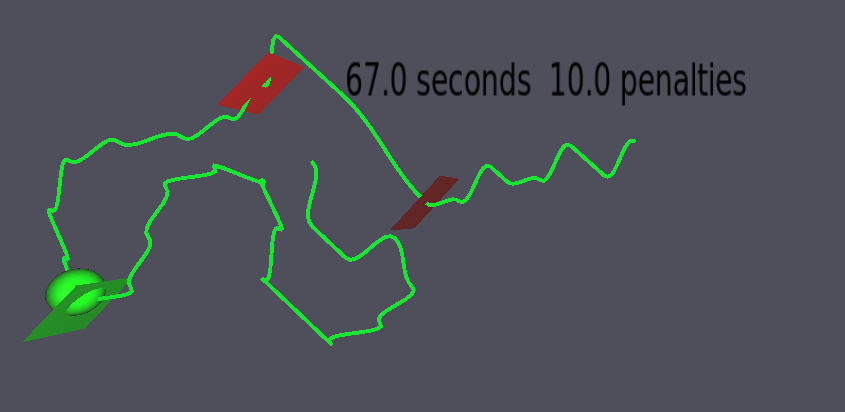
\includegraphics[width=.75\linewidth]{./images/successfulchallenge.png}
		\caption{Line drag use case. The green ball is the handle, red planes are failed challenges and green planes are sucessfully completed challenges.}
	\end{subfigure}
	\begin{subfigure}{\textwidth}
		\centering
		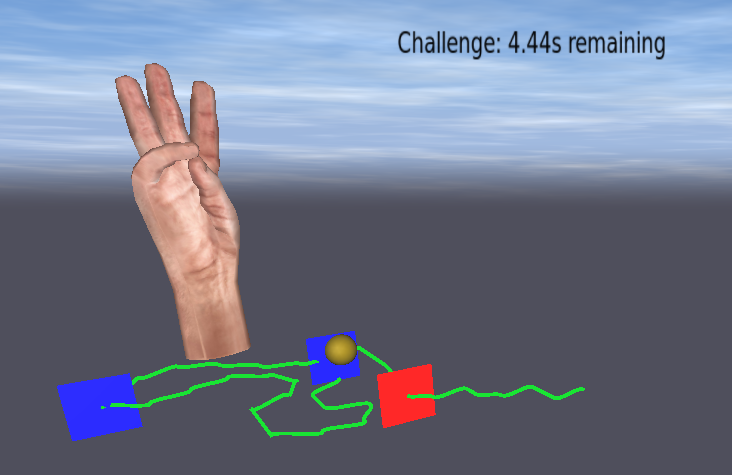
\includegraphics[width=.75\linewidth]{./images/challenge2.png}
		\caption{During a challenge, the remaining time is shown, the handle changes color according to the remaining time (and fades from green to red), and the hand, which has to be mimiced is being shown.}
	\end{subfigure}
	\begin{subfigure}{.5\textwidth}
		\centering
		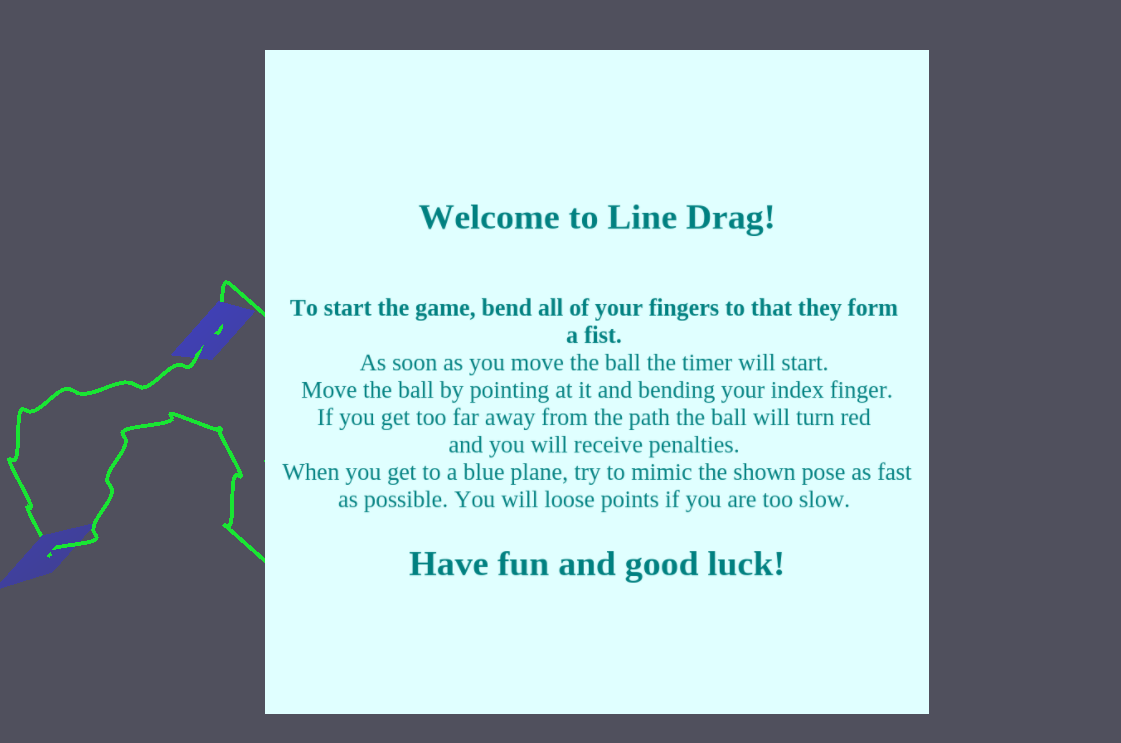
\includegraphics[width=.95\linewidth]{./images/welcome.png}
		\caption{Before the game starts, an intro message is shown.}
	\end{subfigure}%
	\begin{subfigure}{.5\textwidth}
		\centering
		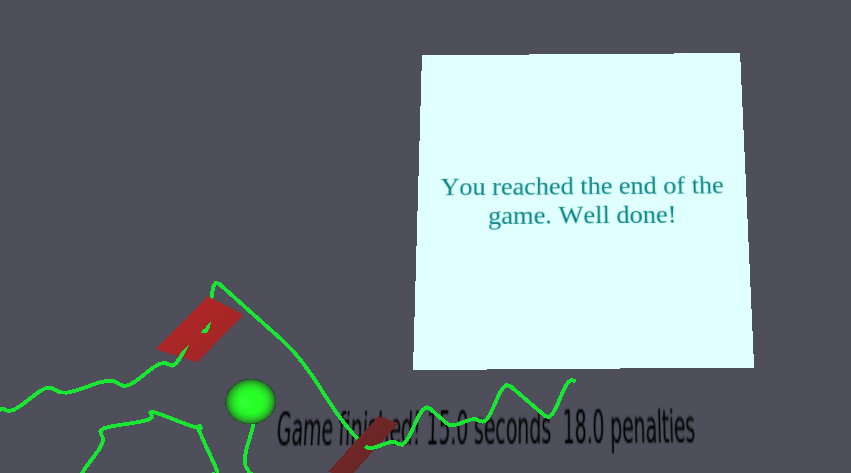
\includegraphics[width=.95\linewidth]{./images/end2.png}
		\caption{Upon sucessfull completion of the game, a end message is shown.}
	\end{subfigure}
	\caption{Line Drag use case.}
	\label{fig:linedragimages}
\end{figure}

\subsection{The towers of Hanoi}
The tower of Hanoi is a mathematical puzzle which contains three pillars and a number of disks. When the game begins, the disks are in ascending order of size stacked on the outer left pillar. The goal of the puzzle is to move the stack from the left to the right pillar only by moving one disk at a time and no disk can be placed on top of a smaller disk. All three pillars can be used to achieve the objective. 

The number of implemented disks in the usecase is three. When the usecase starts the user finds himself in a small room with a table in front of him. The pillars with the disks stand on top of the table. The table itself was downloaded from \url{https://www.turbosquid.com}. The pillars and disks were designed in Blender. At first there was a problem with importing the model into PolyVR because there was no material assigned to the single parts of the models. The second challenge was to apply the physics engine to the objects. When we tried to use the standard \texttt{object.physicalize()} method with the parameters "convex" and "concave" there was a collision box rendered around the disks but it did not cut out the hole in the middle of the disks. Due to this missing hole the disks could not be put onto the pillars. With the help of Victor we could solve the problem by setting the physicalize parameter to "ConvexDecomposed" and changing the ConvexDecomposed parameters via trial and error to working values. The disks can be grabbed by the cyberglove. Since we already had the code for handling the cyberglove in PolyVR for the linedrag usecase, we just use the same code for the tower of Hanoi. In the end I wanted to implement a number of user interfaces for interaction but had no time to finish them because of the problems with the circuit board. In the future there could be functions to select the number of disks to play with or an algorithm which detects when you finish the game or broke the rules. 

\begin{figure}[!h]
	\centering
	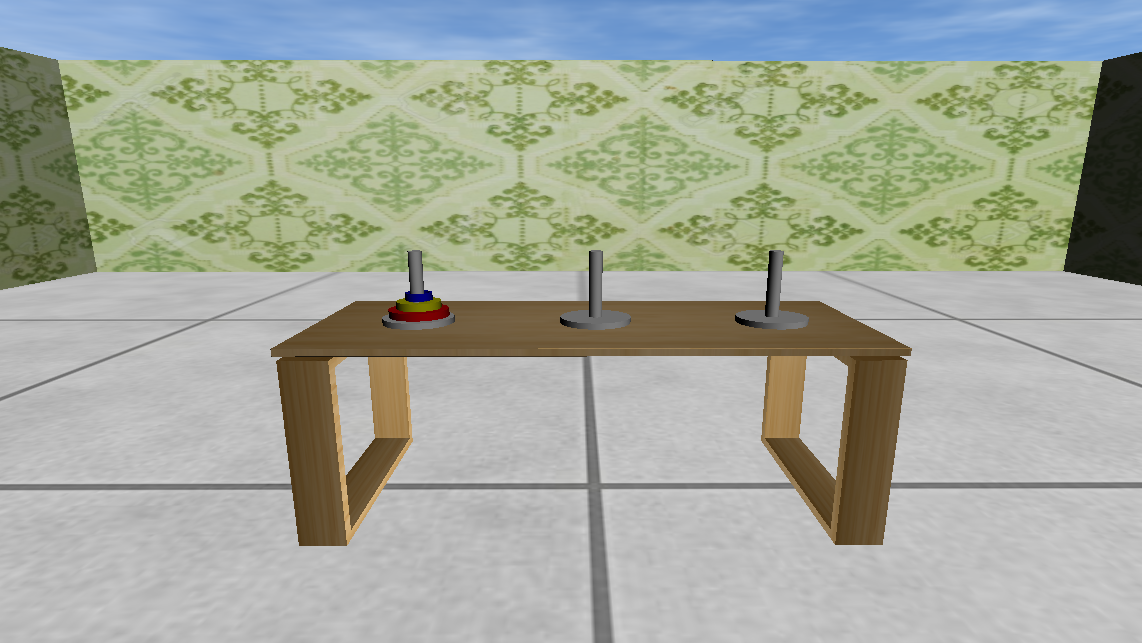
\includegraphics[width=\textwidth]{./images/hanoi2.png}
	\caption{The towers of Hanoi use case}
	\label{hanoi}
\end{figure}

\subsection{Menu}
This use-case consists of several screens, designed with Blender, and arranged on two rows. The ones in the upper row are where web contents are presented and the bottom ones contain buttons to help the user switch between websites. There is also a virtual keyboard added to the scene to help the user type in text editing sections of the webpages, by merely using the Cyberglove.

The screens have both a cover and a face. The webpages and the buttons are designed and presented on the faces. This is done through a localhost. The buttons are designed by HTML as websites and then presented on the faces of the screens through a local server. These buttons are called and recognized by the initial code and accordingly they order the respective page to open on the respective page.

The virtual keyboard was in the beginning designed to write and function within another window, called Textarea. Despite of the many tries, allowing the keyboard to write on the webpages was not met with success. So the keyboard was changed to a simpler one, which contains a text area within its window. It is possible to copy the text written in this text area by means of a simple HTML code which could be applied to a button named „Copy Text“ on the keyboard itself. Again, to go to another webpage and to paste that text without the physical keyboard was not possible. Therefore, the virtual keyboard in this use-case is merely to write a text and exhibit the cyberglove’s ability to fulfill this purpose.

\begin{figure}[!h]
	\centering
	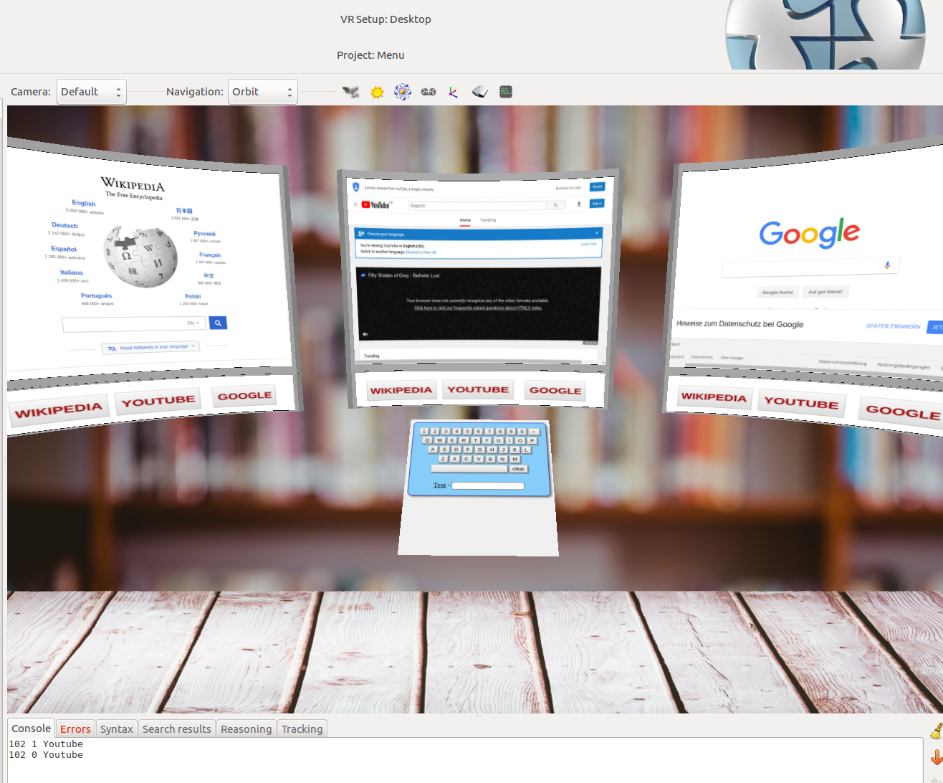
\includegraphics[width=.8\textwidth]{./images/shant/image1.png}
	\caption{Menu use case}
\end{figure}

\subsection{Fruit versus Fastfood}

This is javascript-based use-case that exhibits the functionality of the Cyberglove in grabbing things and moving them around. The game was built according to a tutorial from a book. A sling is grabbed, pulled, directed toward the target, and then released.

There are two levels in the game. It is very similar to the famous game “Angry Birds”, but here fruits are fighting the fast food items. One should throw a fruit by means of a sling and bring down the construction that holds the fast food items within. The game level is won when all the fast food items are disappeared from the screen. The game is lost when the fruits have disappeared before the fast food items.

The issue here was that the game ran on Mozilla browser, but not in the browser within PolyVR. The problem was solved by changing the expression "let" with "var" within the Javascript, and by disabling the audio lines within the code.

\begin{figure}[!h]
	\centering
	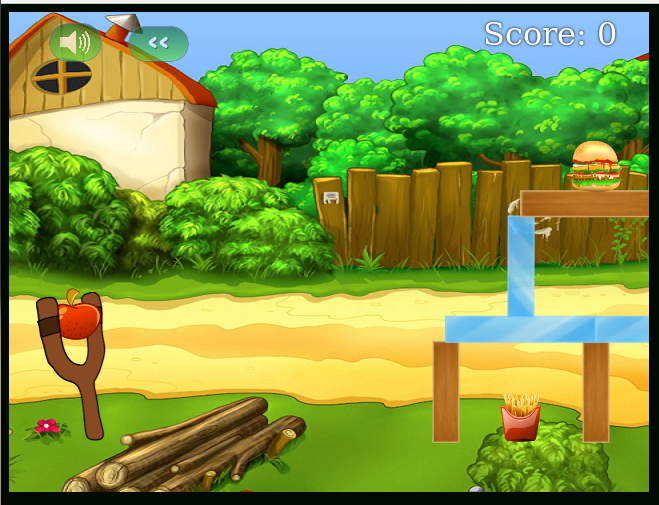
\includegraphics[width=.8\textwidth]{./images/shant/image2.png}
	\caption{``Fruit vs Fastfood'' use case}
\end{figure}

\subsection{Maze}

This was supposed to be 3D game, where a board could be tilted to make a ball move within a maze and be directed toward the exit.

The object was designed in Blender and exported and integrated within PolyVR, then physicalized.
To make the tilting possible a cone was situated below the board, also via Blender, and was programmed so that its pointed head functions as a joint, which allows the board to tilt freely. This joint did not function as planned and the game could not be played, despite many tries and follow-ups.

\begin{figure}[!h]
	\centering
	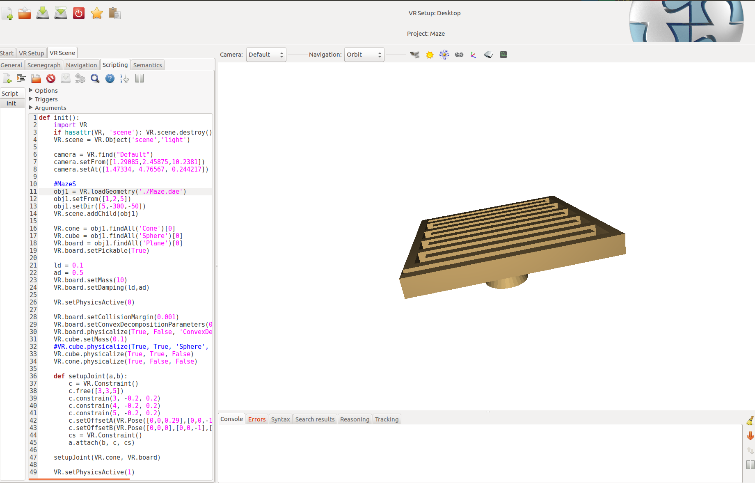
\includegraphics[width=.8\textwidth]{./images/shant/image3.png}
	\caption{Maze use case}
\end{figure}

\subsection{Breakout}

A JavaScript game called Breakout, that uses collision detection to find out when the ball hits the walls or the bricks, and a paddle is moved through the screen by following the mouse pointer or the Cyberglove location in the Cave.

This was built by following a JavaScript tutorial. The ball movement was programmed so that in every instance it draws a new ball and removes the old, so that shadows will not remain behind. The bricks will disappear once collided with the ball. The mouse movement was integrated so that the paddle follows the mouse cursor, without pressing any buttons. And one has 3 tries before the game is over.

Some minimal errors appeared and were fixed.

\begin{figure}[!h]
	\centering
	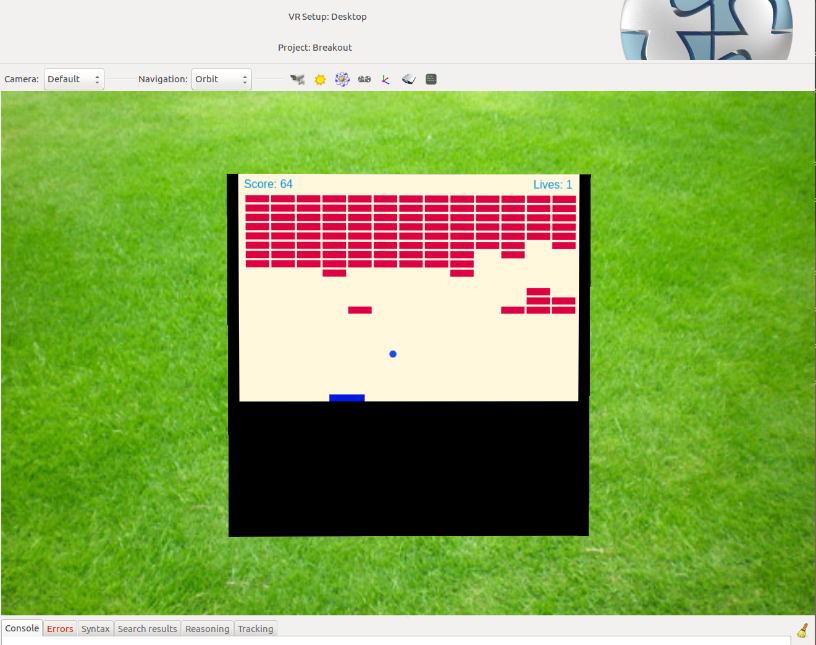
\includegraphics[width=.7\textwidth]{./images/shant/image4.png}
	\caption{Breakout use case}
\end{figure}

\subsection{WireLoop}

To build this use-case it was necessary to get familiar with game physics. I have read about game physics, collision detection, rigid and solid bodies, degrees of freedom etc. Most of the physics engines online have their software and they use functions that work on their software, which cannot be applied in PolyVR directly. PolyVR has its own functions that one has to get familiar with by asking and trying. The drawings were done in Blender and exported to Collada, then integrated in PolyVR and were physicalized. However, this use-case did not reach its final goal because we could not find a way to make it work as hoped. 
We could not make a 3D object (ring) move along a path with simultaneous roation around its own center.
%move a 3D object (ring) along a path (curved tube) with simultaneous rotation around its own center. 
%The mash collision detection gives the collision point and this could be used to program further and improve the use-case.

\begin{figure}[!h]
	\centering
	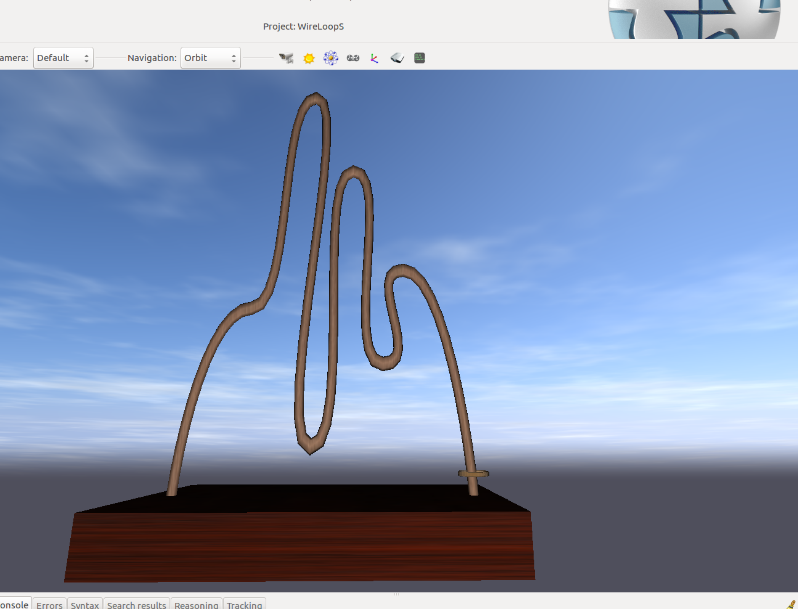
\includegraphics[width=.8\textwidth]{./images/shant/image5.png}
	\caption{WireLoop use case}
\end{figure}


\subsection{Ball play}

The ball play is a tiny physics game. It has a ball, a slidingboard and number of cans. The ball is pickable, the user can pick it and drop it upon the slidingboard. This movement can give the ball a speed in the 3D space, which can be used to throw down the cans. The goal of this game is to throw down as many cans as possible.

The number of implemented cans in the usecase is ten, there is also one sliding board, one ball, and a table. When the usecase starts the user finds himself in a small room with a table in front of him. All of them have been setted in a good sight, which can be easily picked and dropped. All of the models were designed in Blender. Because it was pretty complicated, Victor helped to design the sliding board in Blender. At first there was a problem with importing the model into PolyVR, because the models did not have a UVMap, so each time PolyVR crashed. After adding the UVMap, it finally worked. 

The second challenge is about how to let the ball fly in the 3D Space. At first I just wanted to throw the ball using a hand, which is the Glove in PolyVR. But therefore an extension to PolyVR's physics model would have had to be implemented, but that was too difficult. So instead, it was decided to add a sliding board to the ucecase. 

The third challenge is adjusting the hight of the sliding board, because at first the ball did not get enough speed to hit the cans. So different weights were added to the ball and cans, making the objects correctly physicalized without friction. Then the ball can hit the cans. At the end, a reset option was implemented and the Cyberglove has been integrated in the use case.

The difficulty of the usecase is to determine how high the ball should be dropped. With different heights the ball will get different speeds, although it can hit the cans with different position and force.

\begin{figure}[!h]
	\centering
	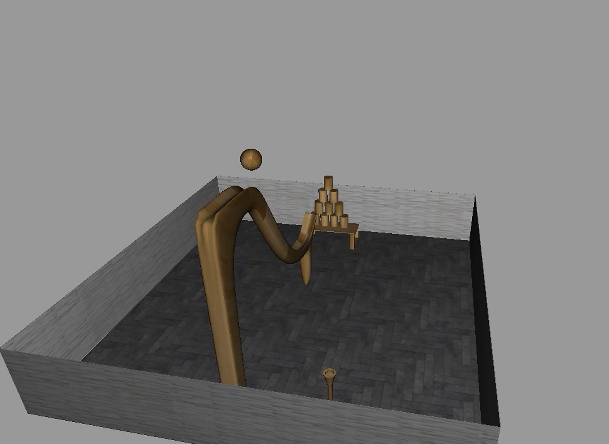
\includegraphics[width=.7\textwidth]{./images/ballplay.png}
	\caption{Ball play use case}
	\label{ballplay}
\end{figure}

\subsection{Glove dragging code}

When creating a new use case, it is very easy to incorperate the glove in order to use it for dragging objects. The following code has to be added as a script into PolyVR which runs on a loop. Objects in PolyVR which are marked as \texttt{Pickable} can then be dragged using the glove.

\lstinputlisting[language=Python,basicstyle=\tiny]{assets/glovedragging.py}